% define \title (only used by writelatex.com)
%\title{CSEC-793 Project Report_Blank}
%%%%%%%%%%%%%%%%%%%%%%%%%%%%%%%%%%%%%%%%%%%%%%%%%%%%%%%%%%%%%%%%%%%%%%
% LaTeX Template: Project Titlepage
%
% Source: http://www.howtotex.com
% Date: April 2011
% 
% This is a title page template which be used for articles & reports.
% 
% Feel free to distribute this example, but please keep the referral
% to howtotex.com
% 
%%%%%%%%%%%%%%%%%%%%%%%%%%%%%%%%%%%%%%%%%%%%%%%%%%%%%%%%%%%%%%%%%%%%%%
% How to use writeLaTeX: 
%
% You edit the source code here on the left, and the preview on the
% right shows you the result within a few seconds.
%
% Bookmark this page and share the URL with your co-authors. They can
% edit at the same time!
%
% You can upload figures, bibliographies, custom classes and
% styles using the files menu.
%
% If you're new to LaTeX, the wikibook is a great place to start:
% http://en.wikibooks.org/wiki/LaTeX
%
%%%%%%%%%%%%%%%%%%%%%%%%%%%%%%%%%%%%%%%%%%%%%%%%%%%%%%%%%%%%%%%%%%%%%%
%
% --------------------------------------------------------------------
% Preamble
% --------------------------------------------------------------------
\documentclass[ fontsize=10pt,twoside]{scrartcl}	% KOMA

\usepackage[letterpaper,pdftex]{geometry}	% A4paper margins
\setlength{\oddsidemargin}{5mm}			% Remove 'twosided' indentation
\setlength{\evensidemargin}{5mm}

\usepackage[english]{babel}
\usepackage[protrusion=true,expansion=true]{microtype}	
\usepackage{amsmath,amsfonts,amsthm,amssymb}
\usepackage{graphicx}
\usepackage{pseudocode}

\usepackage[latin1]{inputenc}
\usepackage{tikz}
\usetikzlibrary{shapes,arrows}
\usetikzlibrary{graphs,graphs.standard}

\usepackage[utf8]{inputenc}
\usepackage[english]{babel}
\usepackage{setspace}
\usepackage[nottoc]{tocbibind}
\usepackage{indentfirst}

\usepackage{tikz}
\newcommand*\circled[1]{\tikz[baseline=(char.base)]{
            \node[shape=circle,draw,inner sep=2pt] (char) {#1};}}

\usepackage[utf8]{inputenc}
\usepackage{tikz}
\usetikzlibrary{arrows}
\usepackage{lipsum}
\tikzset{
    bctleft/.style={.},
    text left/.style={bctleft/.append style={#1}},
    bctright/.style={.},
    text right/.style={bctright/.append style={#1}},
}
\newcommand\bicolortext[2][]{%
    \tikz[baseline=(n.base),inner sep=0pt,outer xsep=0pt,#1]{
      \node(n){\phantom{#2}};
      \foreach \a/\c in {north west/bctleft,south east/bctright}{
        \begin{scope}
          \clip(n.south west)--(n.\a)--(n.north east)--cycle;
          \node[\c]at(n){#2};
        \end{scope}
      }}}
            
\newtheorem{theorem}{Theorem}
\newtheorem{proposition}{Proposition}
\newtheorem{lemma}{Lemma}
\newtheorem{corollary}{Corollary}
\newtheorem{definition}{Definition}
\newtheorem{fact}[theorem]{Fact}
\newtheorem{example}[theorem]{Example}
\newtheorem{open}[theorem]{Open Question}
            




% --------------------------------------------------------------------
% Definitions (do not change this)
% --------------------------------------------------------------------
\newcommand{\HRule}[1]{\rule{\linewidth}{#1}} 	% Horizontal rule




\makeatletter							% Title
\def\printtitle{%						
    {\centering \@title\par}}
\makeatother									

\makeatletter							% Author
\def\printauthor{%					
    {\centering \Large \@author}}				
\makeatother							

% --------------------------------------------------------------------
% Metadata (Change this)
% --------------------------------------------------------------------
\title{	\Large \textsc{ Student Research and Creative Activity \\
Engineering Science and Math \\
Spring Symposium} 	% Subtitle
		 	\\[2.0cm]								% 2cm spacing
			\HRule{2pt} \\						% Upper rule
			\LARGE \textbf{\uppercase{Coloring the Integers: Pseudo Progressions and Ramsey Theory}}	% Title
			\HRule{2pt} \\ [2cm]		% Lower rule + 0.5cm spacing
			\Large \today			% Todays date
		}

 \author{
		Morgan Throckmorton\\
		Major: Applied Mathematics\\
		Department of Mathematics and Statistics\\	
		California State University, Sacramento\\
        morganthrockmorton@csus.edu \\
}


\begin{document}
% ------------------------------------------------------------------------------
% Maketitle
% ------------------------------------------------------------------------------
\thispagestyle{empty}		% Remove page numbering on this page

\printtitle					% Print the title data as defined above
  	\vfill
\printauthor				% Print the author data as defined above
\newpage
% ------------------------------------------------------------------------------
% Begin document
% ------------------------------------------------------------------------------
%\setcounter{page}{1}		% Set page numbering to begin on this page
%\include{abstract}
%\include{introduction}
%\include{conclusion}
%\include{acknowledgement}
%\include{references}
%-------------------------------------------------------------------------------
%\tableofcontents

%In Ramsey Theory, Van der Waerden's theorem states that if you color the integers $r$ distinct colors, there exists a smallest positive integer $N$ such that for any coloring, there exists a $k$-term monochromatic arithmetic progression. 

%Using this idea, we asked ourselves if we loosened the restrictions on the progression by allowing for more than one distinct difference, call it a pseudo progression, 

%we defined an $m$-pseudo progression as a list of increasing integers $a_1,a_2,a_3,...,a_{\ell}$ from $\mathbb{N}$ for which there exists a 

 \newpage
\section{Summary}
\doublespacing 
Suppose you are at a party with six people and you ask yourself the question, is it true that there are at least three people at that party who are either mutual strangers or mutual acquaintances? As it turns out, thanks to the research efforts of Frank Plumpton Ramsey in 1928, not only is this the case, but there is a mathematical reasoning behind it [2]. To visualize this, consider these people as six distinct vertices on a graph all connected to each other with a line, creating an edge, and then color each of these edges one of two distinct colors like the figure below.
\begin{center}
    %\begin{tikzpicture}[scale=2]
% Nodes
%\def \A {(1,0)};
%\def \B {(0.5,0.866)};
%\def \C {(-0.5,0.866)};

%\def \D {(-1,-0)};
%\def \E {(-0.5,-0.866)};
%\def \F {(0.5,-0.866)};
% edges, each separately, change thick/etc
%\draw[red, line width=0.15mm] \A -- \B;
%\draw[blue, line width=0.5mm] \B -- \C -- \E -- \A;
%\draw[red, line width=0.15mm] \D -- \F -- \B;
%
%\node[draw, circle, fill=white] at \A {1};
%\node[draw, circle, fill=white] at \B {2};
%\node[draw, circle, fill=white] at \C {3};
%\node[draw, circle, fill=white] at \D {4};
%\node[draw, circle, fill=white] at \E {5};
%\node[draw, circle, fill=white] at\F {6};
%\end{tikzpicture}
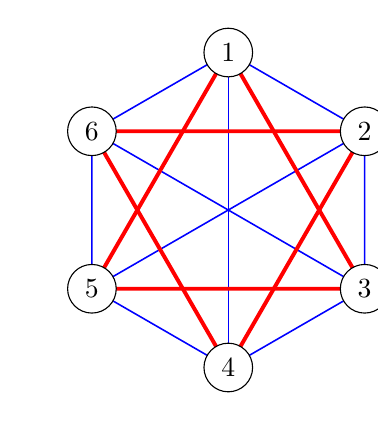
\begin{tikzpicture}[scale=2]
% Nodes
\def \A {(0,1)};
\def \B {(0.866,0.5)};
\def \C {(0.866,-.5)};
\def \D {(0,-1)};
\def \E {(-0.866,-0.5)};
\def \F {(-0.866,0.5)};

% edges, each separately, change thick/etc
\draw[blue, line width=0.2mm] \A -- \B -- \C -- \D -- \E --\F -- \A;
\draw[blue, line width=0.2mm] \A -- \D;
\draw[blue, line width=0.2mm] \B -- \E;
\draw[blue, line width=0.2mm] \C -- \F;
\draw[red, line width=0.5mm] \A -- \C -- \E -- \A;
\draw[red, line width=0.5mm] \B -- \D -- \F -- \B;
%
\node[draw, circle, fill=white] at \A {1};
\node[draw, circle, fill=white] at \B {2};
\node[draw, circle, fill=white] at \C {3};
\node[draw, circle, fill=white] at \D {4};
\node[draw, circle, fill=white] at \E {5};
\node[draw, circle, fill=white] at\F {6};
\end{tikzpicture}
\end{center}
%\begin{center}
%\begin{tikzpicture}
  %\graph { subgraph K_n [n=6,clockwise,radius=2cm] };
%\end{tikzpicture}
%\end{center}
Let's say a thin edge colored blue between two people represents an acquaintance and a thick edge colored red between two people represents two strangers. Notice the red triangles formed by vertices $1,3,5$ and $2,4,6$. These triangles represent three people who then are all mutual strangers, and this isn't a coincidence. What Ramsey proved in his theorem was that now matter how this graph is distinctly colored with two colors, there will always exist a monochromatic triangle between three vertices. Translated to our party problem: at a party with six people, you will always be able to find three people who are either mutual acquaintances or mutual strangers.

This problem is an example from a mathematical field of research known as Ramsey theory which essentially studies how order can be found in randomness. Our research specifically pertains to van der Waerden's theorem which states that if you colored the positive integers with $r$ distinct colors, there exists a least positive integer $n$, denoted $W(k,r)$, such that every coloring of $1,2,\ldots,n$ has a monochromatic $k$-term arithmetic progression [1]. An arithmetic progression can be defined as a list of numbers such that the difference between any two consecutive numbers is separated by one common distance. To illustrate this, let us consider $W(3,2)$. As proved by van der Waerden, $W(3,2) = 9$, that is, for any coloring of $1,\ldots,9$, there will always be a $3$-term monochromatic arithmetic progression. Take for example the following coloring of $1,\ldots,8$. Note that there does not exist a $3$-term monochromatic arithmetic progression, but by adding either a blue $9$ or a red $9$, we can find the following progressions.
\begin{center}
\Large
\textcolor{blue}{\textbf{1 }}\textcolor{red}{2 }\textcolor{red}{3 }\textcolor{blue}{\textbf{4 }}\textcolor{blue}{\textbf{5 }}\textcolor{red}{6 }\textcolor{red}{7 }\textcolor{blue}{\textbf{8}}
\end{center}
\begin{center}
\begin{tikzpicture}[thick]
\draw[blue, ->](0,-1) -- (-3,-3);
\draw[red, ->] (0,-1) -- (3,-3)
\end{tikzpicture}\\
\begin{tabular}{c c c c c c c c}
\Large
   \textcolor{blue}{\textbf{\circled{1} }}\textcolor{red}{2 }\textcolor{red}{3 }\textcolor{blue}{\textbf{4 }}\textcolor{blue}{\textbf{\circled{5} }}\textcolor{red}{6 }\textcolor{red}{7 }\textcolor{blue}{\textbf{8 }}\textcolor{blue}{\textbf{\circled{9}}} & & & & & & & \Large \textcolor{blue}{\textbf{1 }}\textcolor{red}{2 }\textcolor{red}{\circled{3} }\textcolor{blue}{\textbf{4 }}\textcolor{blue}{\textbf{5 }}\textcolor{red}{\circled{6} }\textcolor{red}{7 }\textcolor{blue}{\textbf{8 }}\textcolor{red}{\circled{9}}
\end{tabular}
\end{center}\\

\noindent On the left, if we color $9$ blue, then we have the blue $3$-term arithmetic progression $1,5,9$ where all consecutive integers are separated by a distance of $4$. On the right, if we color $9$ red, then we have the red $3$-term arithmetic progression $3,6,9$ where all consecutive integers are separated by a distance of $3$. Many other variations of this same problem have been studied and for our research we strive to study how the introduction of pseudo progressions affect this number $n$. 

%In this summary, I will introduce our proposed research questions, disclose our approach to solving these questions, and reveal where we are at currently in our research and the direction we intend to take next.
%-----> NEED TO ADD ARROWS <-------------
%\begin{center}
%\Large
%\textcolor{blue}{\textbf{1 }}\textcolor{red}{2 }\textcolor{red}{3 }\textcolor{blue}{\textbf{4 }}\textcolor{blue}{\textbf{5 }}\textcolor{red}{6 }\textcolor{red}{7 }\textcolor{blue}{\textbf{8}} \tikzset{text left=blue,text right=red}\bicolortext[transform shape]{9}
%\end{center}
%---------> Original Introduction <------------------------
%Within the branch of combinatorics in mathematics comes Ramsey Theory, which can best be defined as the examination of how set partitions preserve the structure of various mathematical objects or properties [1]. The field of research is named after Frank Plumpton Ramsey, whom in 1928 proved what is known today as Ramsey's theorem that answered illustrious problems such as the "party puzzle" [2]. which asks that at any given part with six people, is it true that three people have all met one another, or three people are strangers [2]? Turns out, thanks to Ramsey's theorem, this is true. Our research specifically pertains to Ramsey Theory on the integers in which we explore Van der Waerden's Theorem. The idea behind Van der Waerden's theorem is that if you colored the positive integers with $r$ distinct colors, there exists a least positive integer $N$ such that for any one of the $r^N$ colorings, there exists a monochromatic $k$-term arithmetic progression [1]. This smallest such $N$ is known as Van der Waerden's number. As a team, we have set out to solve other variations of this type of Ramsey problem, introducing what we define as pseudo progressions. In this summary, I will introduce our proposed research questions, disclose our approach to solving the problem, and reveal where we are at currently in our research and the direction we intend to take next.
%-------------> Original Introduction <--------------------

Since van der Waerden's theorem only applies to arithmetic progressions, we proposed to study what happens if we allow a single progression to have up to $m$ common differences. Recall that in our previous example, the coloring of $1,\ldots,8$ did not contain a $3$-term monochromatic arithmetic progression. Since an arithmetic progression has at most $1$ distinct common difference, how would allowing for $2$ distinct common differences have an impact on that same coloring? By observing that same coloring, we look for progressions that contain at most $2$ distinct differences.
\begin{center}
    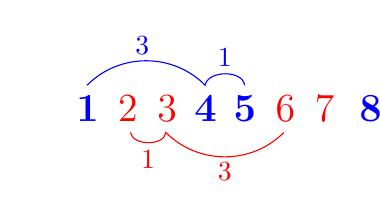
\begin{tikzpicture}[scale=1]
%-------->nodes<--------------
\node at (0,0) {\Large\textcolor{blue}{\textbf{1 }}}; % 1
\node at (0.5,0) {\Large\textcolor{red}{2 }}; % 2
\node at (1,0) {\Large\textcolor{red}{3 }}; %3
\node at (1.5,0) {\Large\textcolor{blue}{\textbf{4 }}}; % 4
\node at (2,0) {\Large\textcolor{blue}{\textbf{5 }}}; % 5
\node at (2.5,0) {\Large\textcolor{red}{6 }}; % 6
\node at (3,0) {\Large\textcolor{red}{7 }}; % 7 
\node at (3.5,0) {\Large\textcolor{blue}{\textbf{8}}}; % 8 
%------------->top arrows<------------------
\draw [blue] (-.1,0.3) to[out=45,in=135] (1.4,0.3) to [out=80,in=96] (1.90,.3); 
%\draw [blue, ->, width=100pt] (1.4,.3) to[out=90,in=90] (1.90,.3);
%----------------> bottom arrows<------------------
\draw [red] (.450,-.3) to [out=-80,in=-96] (.90,-.3) to[out=-45 ,in=-135 ] (2.4,-.3);
%-----------> top nodes <---------------
\node at (0.60,.80) {\textcolor{blue}{3}};
\node at (1.65,.65) {\textcolor{blue}{1}};
%-------------> bottom nodes <-----------------
\node at (.675,-.65) {\textcolor{red}{1}};
\node at (1.65,-.80) {\textcolor{red}{3}};
\end{tikzpicture}
\end{center}
%\begin{center}
%\Large
%\textcolor{blue}{\textbf{1 }}\textcolor{red}{2 }\textcolor{red}{3 }\textcolor{blue}{\textbf{4 }}\textcolor{blue}{\textbf{5 }}\textcolor{red}{6 }\textcolor{red}{7 }\textcolor{blue}{\textbf{8}}
%\end{center}
Above we have the blue $3$-term $2$-pseudo progression $1,4,5$ where  consecutive integers are separated by a distance of $1$ or $3$ and below we have the red $3$-term $2$-pseudo progression $2,3,6$ where consecutive integers are separated by a distance of $1$ or $3$. Thus let us define a $k$-term $m$-pseudo progression as a list of increasing integers $a_1,a_2,\ldots,a_k$ from $\mathbb{N}$ for which there exists a set $\{d_1,d_2,\ldots,d_{m}\}$ such that $a_{i+1} - a_i \in \{d_1,d_2,\ldots,d_{m}\}$ for all $i \in \mathbb{N}$. We will then define $B_m(k,r)$ to be the smallest positive integer $n$ for which every $r$-coloring contains a $k$-term $m$-pseudo progression. It is worth noting that the set of all $(m-1)$-pseudo progressions are a subset of the set of all $m$-pseudo progressions since we do not require that the progression have exactly $m$ distinct differences---we require that it contains at most $m$ distinct differences. Since van der Waerden proved that $W(k,r)$ exists and by our example we must have $B_m(k,r) \leq W(k,r)$, we know that $B_m(k,r)$ exists. Since we know that this exists, our research goal is to prove several precise values of $B_m(k,r)$ for small values of $k$, $m$, and $r$ and to find general bounds for all values of $k$, $m$, and $r.$

Over a century of research suggests that finding an explicit formula for $B_m(k,r)$ is nearly impossible, so we look to prove small cases and general bounds by using integer partitions. Included below is a table of some of the known values of of $B_m(k,2)$ that we have found during our research. Currently we have restricted our research to looking at colorings with at most two distinct colors. Note that the first row with $m = 1$ are simply van der Waerden's numbers of arithmetic progressions with two distinct colors.

\begin{center}
\begin{tabular}{ | m | m | m | m | m | m | m | m | m | m | m |  } 
\hline
$m\backslash k$& 1 & 2 & 3 & 4 & 5 & 6 & 7 & 8 & 9 & 10  \\ 
\hline
1 & 1 & 3 & 9 & 35 & 178  & 1132 & $>$3703  & $>$11,495 & $>41,265$  & $>$103,474   \\ 
\hline
2 & 1 & 3 & 5 & 9 & 14 & $>13$ & $>13$ & $>14$ & $>16$ & $>18$\\
\hline
3 & 1 & 3 & 5 & 7 & 9 & 11 & $>14$ & $>14$ & $>16$ & $>18$ \\
\hline
4 & 1 & 3 & 5 & 7 & 9 & 11 & 13 & 15 & 17 & 19  \\
\hline
5 & 1 & 3 & 5 & 7 & 9 & 11 & 13 & 15 & 17 & 19  \\
\hline
6 & 1 & 3 & 5 & 7 & 9 & 11 & 13 & 15 & 17 & 19 \\ 
\hline

\end{tabular}
\end{center}\\

\noindent As the table suggests, as we decrease the restrictions on the progression by allowing for an increase in $m$ distinct differences, $B_m(k,2)$ becomes much easier to find. The majority of our approach has involved the use of integer partitions combined with targeted elements of brute force that require checking individual colorings for various $m$-pseudo progressions. To demonstrate how we used integer partitions to look for small values, we include the following proof of $B_2(4,2) = 9$.

\begin{theorem}
$B_2(4,2) = 9$
\end{theorem}
\begin{proof}
First let us consider the following coloring: 
%------> USE ARROWS HERE <-------
\begin{center}
    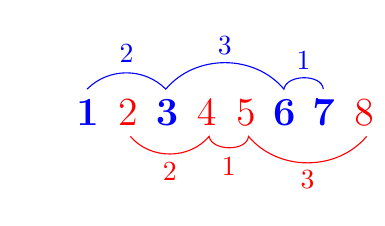
\begin{tikzpicture}[scale=1]
%-------->nodes<--------------
\node at (0,0) {\Large\textcolor{blue}{\textbf{1 }}}; % 1
\node at (0.5,0) {\Large\textcolor{red}{2 }}; % 2
\node at (1,0) {\Large\textcolor{blue}{\textbf{3} }}; %3
\node at (1.5,0) {\Large\textcolor{red}{4 }}; % 4
\node at (2,0) {\Large\textcolor{red}{5 }}; % 5
\node at (2.5,0) {\Large\textcolor{blue}{\textbf{6 }}}; % 6
\node at (3,0) {\Large\textcolor{blue}{\textbf{7 }}}; % 7 
\node at (3.5,0) {\Large\textcolor{red}{8 }}; % 8 
%------------->top arrows<------------------
\draw [blue] (-.1,0.3) to[out=45,in=135] (.90,.3) to [out=50,in=130] (2.40,.3) to [out=80,in=95] (2.90,.3); 
%\draw [blue, ->, width=100pt] (1.4,.3) to[out=90,in=90] (1.90,.3);
%----------------> bottom arrows<------------------
\draw [red] (.450,-.3) to [out=-50,in=-130] (1.45,-.3) to[out=-80 ,in=-95] (1.95,-.3) to [out=-50,in=-130] (3.45,-.3);
%-----------> top nodes <---------------
\node at (0.40,.75) {\textcolor{blue}{2}};
\node at (1.65,.85) {\textcolor{blue}{3}};
\node at (2.65,.658) {\textcolor{blue}{1}};
%-------------> bottom nodes <-----------------
\node at (.95,-.75) {\textcolor{red}{2}};
\node at (1.7,-.68) {\textcolor{red}{1}};
\node at (2.7,-.85) {\textcolor{red}{3}};
\end{tikzpicture}
\end{center}
%begin{center}
%large
%textcolor{blue}{\textbf{1 }}\textcolor{red}{2 }\textcolor{blue}{\textbf{3 }}\textcolor{red}{4 }\textcolor{red}{5 }\textcolor{blue}{\textbf{6 }}\textcolor{blue}{\textbf{7 }}\textcolor{red}{8}
%end{center}
We use this as a counter example to show that $B_2(4,2) \neq 8$. Since we are looking for monochromatic $4$-term progressions with at most $2$ distinct common differences and both $4$-term monochromatic progressions in the given coloring have $3$ distinct differences, it must be that $B_2(4,2)>8$.

%Since we are looking for $4$-term progressions with at most $2$ distinct differences and both $4$-term monochromatic progressions in the given coloring have $3$ distinct differences, we have found a specific coloring of $1,\ldots,8$ that does not have one. %Therefore it is not true that every coloring has such a progression and it must be that $B_2(4,2) \neq 8$. 


%Since the only $4$-term monochromatic progressions are $1,3,6,7$ and $2,4,5,8$ and neither of those are $2$-pseudo progressions, we conclude that $B_2(4,2) \neq 8$. Now, let us choose to color the numbers $1-9$ either blue or red and define the number of blue colorings as $b$ and the number of red colorings as $r$ and assume without loss of generality that $r \leq b$. Since we are looking at the integers $1-9$, the first case we must consider is $b = 5$ and $r = 4$. 



So, let us choose to color all the integers in $1,\ldots,9$ either red or blue and define the number of integers colored blue as $b$ and the number of integers colored red as $r$ and assume without loss of generality $r\leq b$. The first case we must consider is $b = 5$ and $r = 4$. From this we will use integer partitions to partition the $5$ blue colors into $5$ distinct parts on the left and the $4$ red colors into $4$ distinct parts on the right.
\begin{flalign*}
\large
5 &=  \textcolor{blue}{\bigcirc}\textcolor{blue}{\bigcirc}\textcolor{blue}{\bigcirc}\textcolor{blue}{\bigcirc}\textcolor{blue}{\bigcirc}  & 4&= \textcolor{red}{\bigcirc}\textcolor{red}{\bigcirc}\textcolor{red}{\bigcirc}\textcolor{red}{\bigcirc} &&\\
2 + 3 &= \textcolor{blue}{\bigcirc}\textcolor{blue}{\bigcirc}\textcolor{white}{\bigcirc}\textcolor{blue}{\bigcirc}\textcolor{blue}{\bigcirc}\textcolor{blue}{\bigcirc} & 2+2 & = \textcolor{red}{\bigcirc}\textcolor{red}{\bigcirc}\textcolor{white}{\bigcirc}\textcolor{red}{\bigcirc}\textcolor{red}{\bigcirc} &&\\
1 + 4 &= \textcolor{blue}{\bigcirc}\textcolor{white}{\bigcirc}\textcolor{blue}{\bigcirc}\textcolor{blue}{\bigcirc}\textcolor{blue}{\bigcirc}\textcolor{blue}{\bigcirc} & 1+3 &= \textcolor{red}{\bigcirc}\textcolor{white}{\bigcirc}\textcolor{red}{\bigcirc}\textcolor{red}{\bigcirc}\textcolor{red}{\bigcirc} &&\\
1 + 2 + 2 &= \textcolor{blue}{\bigcirc}\textcolor{white}{\bigcirc}\textcolor{blue}{\bigcirc}\textcolor{blue}{\bigcirc}\textcolor{white}{\bigcirc}\textcolor{blue}{\bigcirc}\textcolor{blue}{\bigcirc} & 1+1+2 &= \textcolor{red}{\bigcirc}\textcolor{white}{\bigcirc}\textcolor{red}{\bigcirc}\textcolor{white}{\bigcirc}\textcolor{red}{\bigcirc}\textcolor{red}{\bigcirc} &&\\
1+1+3 &=  \textcolor{blue}{\bigcirc}\textcolor{white}{\bigcirc}\textcolor{blue}{\bigcirc}\textcolor{white}{\bigcirc}\textcolor{blue}{\bigcirc}\textcolor{blue}{\bigcirc}\textcolor{blue}{\bigcirc} & 1+1+1+1 &= \textcolor{red}{\bigcirc}\textcolor{white}{\bigcirc}\textcolor{red}{\bigcirc}\textcolor{white}{\bigcirc}\textcolor{red}{\bigcirc}\textcolor{white}{\bigcirc}\textcolor{red}{\bigcirc}  &&\\
1+1+1+2 &= \textcolor{blue}{\bigcirc}\textcolor{white}{\bigcirc}\textcolor{blue}{\bigcirc}\textcolor{white}{\bigcirc}\textcolor{blue}{\bigcirc}\textcolor{white}{\bigcirc}\textcolor{blue}{\bigcirc}\textcolor{blue}{\bigcirc} &&\\
1+1+1+1+1 &= \textcolor{blue}{\bigcirc}\textcolor{white}{\bigcirc}\textcolor{blue}{\bigcirc}\textcolor{white}{\bigcirc}\textcolor{blue}{\bigcirc}\textcolor{white}{\bigcirc}\textcolor{blue}{\bigcirc}\textcolor{white}{\bigcirc}\textcolor{blue}{\bigcirc}
\end{flalign*}
We view the red and blue circles as colorings of a list of numbers, but in no particular order. Our goal will be to interweave the blue parts with corresponding red parts and then consider all possible permutations that will give us distinct colorings. We will first begin by looking for blue $2$-pseudo progressions because if we can find a blue $2$-pseudo progression within every coloring for $b = 5$ and $r=4$, every other coloring will contain a blue $2$-pseudo progression with $r\leq b$. If we cannot find a blue $2$-pseudo progression for every coloring such that $b = 5$ and $r = 4$, we will have to look at the subsequent cases for $b > 5$ and $r < 4$. 
%First, let us introduce a lemma that will justify why we will choose to look for $2$-pseudo progressions for one color first, rather than considering both colors.
%\begin{lemma}
%Let the number of blue colorings be defined as $b$ and the number of red colorings be defined as $r$ and assume without loss of generality that $r \leq b$. If there exists a blue $m$-pseudo progression in every coloring for $b = x$ and $r = y$, for $x,y \in \mathbb{N}$, then every coloring for which $b = x + i$ and $r = y-i$ will also contain a blue $m$-pseudo progression for all $i \in \mathbb{N}$.
%\end{lemma}

Our next step will be to eliminate partitions that will always contain a blue $2$-pseudo progression and to do so we will introduce a lemma.
\begin{lemma}
Suppose you are looking at any integer partition. If for some $k$-length $m$-pseudo progression, the sum of $m$ parts is greater than or equal to $k$, then you are guaranteed a monochromatic $m$-pseudo progression of length $k$.
\end{lemma}
%\noindent Since we have more blue numbers colored than red numbers, it makes sense to look for blue $2$-pseudo progressions first since if we can find a blue $2$-pseudo progression within every such coloring, by our lemma every other possible coloring will contain a blue $2$-pseudo progression. The proof of this is actually quite simple. If you can prove that every coloring of $b=5$ and $r = 4$ contains a blue $2$-pseudo progression, then if you picked any integer colored red and switched it to blue, clearly it would still contain the same blue $2$-pseudo progression. Since we want to look only at the blue partitions, our second lemma will allow us to eliminate blue partitions that already contain a $2$-pseudo progression.
\noindent What this means for us is if the sum of any two parts of any blue partition adds up to $4$, by our lemma that partition will contain a $2$-pseudo progression. Consider the following example of the partition $2+2+1$ permuted in the order $2+1+2$.
%------>ADD ARROWS HERE <--------
\begin{center}
    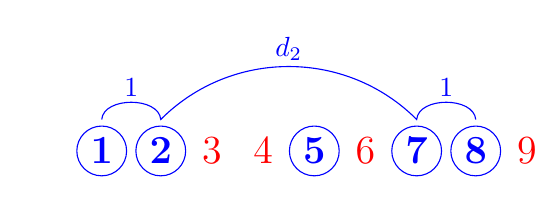
\begin{tikzpicture}[scale=1]
%-------->nodes<--------------
\node at (0,0) {\Large\textcolor{blue}{\textbf{\circled{1}}}}; % 1
\node at (.75,0) {\Large\textcolor{blue}{\textbf{\circled{2}}}}; % 2
\node at (1.40,0) {\Large\textcolor{red}{3}}; %3
\node at (2.05,0) {\Large\textcolor{red}{4}}; % 4
\node at (2.7,0) {\Large\textcolor{blue}{\textbf{\circled{5}}}}; % 5
\node at (3.35,0) {\Large\textcolor{red}{6}}; % 6
\node at (4,0) {\Large\textcolor{blue}{\textbf{\circled{7}}}}; % 7 
\node at (4.75,0) {\Large\textcolor{blue}{\textbf{\circled{8}}}};% 8 
\node at (5.4,0) {\Large\textcolor{red}{9}};
%------------->top arrows<------------------
\draw [blue] (0,.4) to [out=85,in=95] (.75,.4) to[out=45,in=135] (4,.4) to[out=85,in=95] (4.75,.4);

%\draw [blue] (-.1,0.3) to[out=45,in=135] (.90,.3) to [out=50,in=130] (2.40,.3) to [out=80,in=95] (2.90,.3); 
%\draw [blue, ->, width=100pt] (1.4,.3) to[out=90,in=90] (1.90,.3);
%----------------> bottom arrows<------------------
%\draw [red] (.450,-.3) to [out=-50,in=-130] (1.45,-.3) to[out=-80 ,in=-95] (1.95,-.3) to [out=-50,in=-130] (3.45,-.3);
%-----------> top nodes <---------------
\node at (.375,.8) {\textcolor{blue}{1}};
\node at (2.375,1.3) {\textcolor{blue}{$d_2$}};
\node at (4.375,.8) {\textcolor{blue}{1}};

%\node at (0.40,.75) {\textcolor{blue}{2}};
%\node at (1.65,.85) {\textcolor{blue}{3}};
%\node at (2.65,.658) {\textcolor{blue}{1}};
%-------------> bottom nodes <-----------------
%\node at (.95,-.75) {\textcolor{red}{2}};
%\node at (1.7,-.68) {\textcolor{red}{1}};
%\node at (2.7,-.85) {\textcolor{red}{3}};
\end{tikzpicture}
\end{center}
%\begin{center}
 %   \textcolor{blue}{\textbf{\circled{1 }}}\textcolor{blue}{\textbf{\circled{2 }}}\textcolor{red}{3 }\textcolor{red}{4 }\textcolor{blue}{\textbf{\circled{5} }}\textcolor{red}{6 }\textcolor{blue}{\textbf{\circled{7 }}}\textcolor{blue}{\textbf{\circled{8 }}}\textcolor{red}{9}
%\end{center}
While we will not always know the distance each part is separated by, taking one ``jump" from one $2$-term arithmetic progression to another $2$-term arithmetic progression gives us a $4$-term $2$-pseudo progression where the difference between every consecutive pair of integers is an element of the set $\{1,d_2\}$ for some unknown $d_2 \in \mathbb{N}$. By using this lemma, we will only need to consider the blue partitions \textcolor{blue}{$1+1+1+1+1$} and \textcolor{blue}{$1+1+1+2$} and all matching red partitions. Assuming $r\leq b$, for any blue partition with $d$ distinct parts, a red partition is a \emph{match} if $d-1 \leq c \leq d+1$ for any red partition with $c$ distinct parts. Thus we have that the blue partition \textcolor{blue}{$1+1+1+1+1$} matches with the red partition \textcolor{red}{1+1+1+1} and the blue partition \textcolor{blue}{$1+1+1+2$} matches with the red partitions \textcolor{red}{$1+1+1+1$} and \textcolor{red}{$1+1+2$}. Next we will choose to fix blue and consider all distinct permutations of blue. Since we only care about finding a monochromatic $2$-pseudo progression, any reflection of blue partitions will be disregarded as it is not considered distinct. By choosing to fix blue, however, we must consider all possible permutations of red partitions. Below, we demonstrate how we start with the blue partition \textcolor{blue}{1+1+1+2} and match it with the following red partitions \textcolor{red}{1+1+2} and \textcolor{red}{1+1+1+1}. Around the outside of the map are all of the possible distinct colorings for the partitions, each marked with a dot inside the circle to show the existence of a $4$-term blue $2$-pseudo progression.
\begin{center}
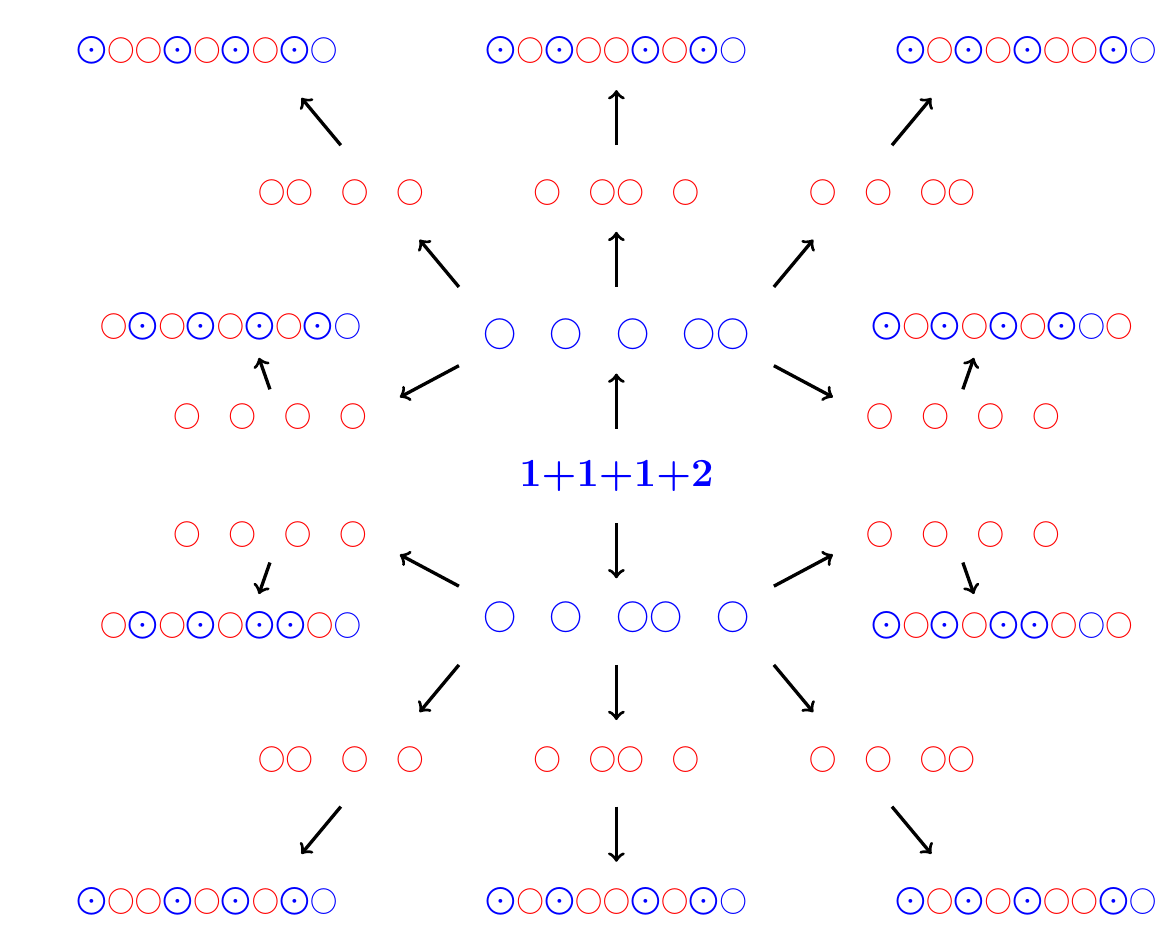
\begin{tikzpicture}
%center box
\node[blue] at (-1,0) {\Large\textbf{1+1+1+2}};
\draw[very thick,-> ] (-1,.6) -- (-1,1.3); % height = .7
\draw[very thick, ->] (-1,-.6) -- (-1,-1.3); % height = -.7

\node at (-1,1.8) {\large$\textcolor{blue}{\bigcirc}\textcolor{white}{\bigcirc}\textcolor{blue}{\bigcirc}\textcolor{white}{\bigcirc}\textcolor{blue}{\bigcirc}\textcolor{white}{\bigcirc}\textcolor{blue}{\bigcirc}\textcolor{blue}{\bigcirc}$}; %height = .5 from last

\node at (-1,-1.8) {\large$\textcolor{blue}{\bigcirc}\textcolor{white}{\bigcirc}\textcolor{blue}{\bigcirc}\textcolor{white}{\bigcirc}\textcolor{blue}{\bigcirc}\textcolor{blue}{\bigcirc}\textcolor{white}{\bigcirc}\textcolor{blue}{\bigcirc}$};

\draw[very thick, ->] (-1,2.4) -- (-1,3.1); % up straight
\draw[very thick, ->] (1,2.4) -- (1.5,3); % up right
\draw[very thick, ->] (-3,2.4) -- (-3.5,3); % up left
\draw[very thick, ->] (-1,-2.4) -- (-1,-3.1); % down straight
\draw[very thick, ->] (1,-2.4) -- (1.5,-3); % down right
\draw[very thick, ->] (-3,-2.4) -- (-3.5,-3); % down left

\draw[very thick, ->] (1,1.4) -- (1.75,1);
\draw[very thick, ->] (1,-1.4) -- (1.75,-1);
\draw[very thick, ->] (-3,1.4) -- (-3.75,1);
\draw[very thick, ->] (-3,-1.4) -- (-3.75,-1);
%\draw[very thick, ->] (-1,1.4) -- (-2.75,1);
%\draw[very thick, ->] (-3,-1.4) -- (3.75,-1);

\node at (3.4,.75) {$\Large\textcolor{red}{\bigcirc}\textcolor{white}{\bigcirc}\textcolor{red}{\bigcirc}\textcolor{white}{\bigcirc}\textcolor{red}{\bigcirc}\textcolor{white}{\bigcirc}\textcolor{red}{\bigcirc}$};

\node at (-5.4,.75) {$\Large\textcolor{red}{\bigcirc}\textcolor{white}{\bigcirc}\textcolor{red}{\bigcirc}\textcolor{white}{\bigcirc}\textcolor{red}{\bigcirc}\textcolor{white}{\bigcirc}\textcolor{red}{\bigcirc}$};

\node at (3.4,-.75) {$\Large\textcolor{red}{\bigcirc}\textcolor{white}{\bigcirc}\textcolor{red}{\bigcirc}\textcolor{white}{\bigcirc}\textcolor{red}{\bigcirc}\textcolor{white}{\bigcirc}\textcolor{red}{\bigcirc}$};

\node at (-5.4,-.75) {$\Large\textcolor{red}{\bigcirc}\textcolor{white}{\bigcirc}\textcolor{red}{\bigcirc}\textcolor{white}{\bigcirc}\textcolor{red}{\bigcirc}\textcolor{white}{\bigcirc}\textcolor{red}{\bigcirc}$};

\draw[very thick, ->] (3.4,1.1) -- (3.54,1.5);
\draw[very thick, ->] (-5.4,1.1) -- (-5.54,1.5);
\draw[very thick, ->] (3.4,-1.1) -- (3.54,-1.5);
\draw[very thick, ->] (-5.4,-1.1) -- (-5.54,-1.5);


\node at (3.9,1.9) {$\Large\textcolor{blue}{\bigodot}\textcolor{red}{\bigcirc}\textcolor{blue}{\bigodot}\textcolor{red}{\bigcirc}\textcolor{blue}{\bigodot}\textcolor{red}{\bigcirc}\textcolor{blue}{\bigodot}\textcolor{blue}{\bigcirc}\textcolor{red}{\bigcirc}$};

\node at (3.9,-1.9) {$\Large\textcolor{blue}{\bigodot}\textcolor{red}{\bigcirc}\textcolor{blue}{\bigodot}\textcolor{red}{\bigcirc}\textcolor{blue}{\bigodot}\textcolor{blue}{\bigodot}\textcolor{red}{\bigcirc}\textcolor{blue}{\bigcirc}\textcolor{red}{\bigcirc}$};

\node at (-5.9,1.9) {$\Large\textcolor{red}{\bigcirc}\textcolor{blue}{\bigodot}\textcolor{red}{\bigcirc}\textcolor{blue}{\bigodot}\textcolor{red}{\bigcirc}\textcolor{blue}{\bigodot}\textcolor{red}{\bigcirc}\textcolor{blue}{\bigodot}\textcolor{blue}{\bigcirc}$};

\node at (-5.9,-1.9) {$\Large\textcolor{red}{\bigcirc}\textcolor{blue}{\bigodot}\textcolor{red}{\bigcirc}\textcolor{blue}{\bigodot}\textcolor{red}{\bigcirc}\textcolor{blue}{\bigodot}\textcolor{blue}{\bigodot}\textcolor{red}{\bigcirc}\textcolor{blue}{\bigcirc}$};

%--------


\node at (-1,3.6) {$\Large\textcolor{red}{\bigcirc}\textcolor{white}{\bigcirc}\textcolor{red}{\bigcirc}\textcolor{red}{\bigcirc}\textcolor{white}{\bigcirc}\textcolor{red}{\bigcirc}$}; % up center

\node at (2.5,3.6) {$\Large\textcolor{red}{\bigcirc}\textcolor{white}{\bigcirc}\textcolor{red}{\bigcirc}\textcolor{white}{\bigcirc}\textcolor{red}{\bigcirc}\textcolor{red}{\bigcirc}$}; % up right

\node at (-4.5,3.6) {$\Large\textcolor{red}{\bigcirc}\textcolor{red}{\bigcirc}\textcolor{white}{\bigcirc}\textcolor{red}{\bigcirc}\textcolor{white}{\bigcirc}\textcolor{red}{\bigcirc}$}; % up left 

\node at (-1,-3.6) {$\Large\textcolor{red}{\bigcirc}\textcolor{white}{\bigcirc}\textcolor{red}{\bigcirc}\textcolor{red}{\bigcirc}\textcolor{white}{\bigcirc}\textcolor{red}{\bigcirc}$}; % down center

\node at (2.5,-3.6) {$\Large\textcolor{red}{\bigcirc}\textcolor{white}{\bigcirc}\textcolor{red}{\bigcirc}\textcolor{white}{\bigcirc}\textcolor{red}{\bigcirc}\textcolor{red}{\bigcirc}$}; % down right

\node at (-4.5,-3.6) {$\Large\textcolor{red}{\bigcirc}\textcolor{red}{\bigcirc}\textcolor{white}{\bigcirc}\textcolor{red}{\bigcirc}\textcolor{white}{\bigcirc}\textcolor{red}{\bigcirc}$}; % down left

\draw[very thick, ->] (-1,4.2) -- (-1,4.9); % up center
\draw[very thick, ->] (2.5,4.2) -- (3,4.8); % up right
\draw[very thick, ->] (-4.5,4.2) -- (-5,4.8); % up left
\draw[very thick, ->] (-1,-4.2) -- (-1,-4.9); % down center
\draw[very thick, ->] (2.5,-4.2) -- (3,-4.8); % down right
\draw[very thick, ->] (-4.5,-4.2) -- (-5,-4.8); % down left

\node at (-1,5.4) {$\Large\textcolor{blue}{\bigodot}\textcolor{red}{\bigcirc}\textcolor{blue}{\bigodot}\textcolor{red}{\bigcirc}\textcolor{red}{\bigcirc}\textcolor{blue}{\bigodot}\textcolor{red}{\bigcirc}\textcolor{blue}{\bigodot}\textcolor{blue}{\bigcirc}$}; % up center 

\node at (4.2,5.4) {$\Large\textcolor{blue}{\bigodot}\textcolor{red}{\bigcirc}\textcolor{blue}{\bigodot}\textcolor{red}{\bigcirc}\textcolor{blue}{\bigodot}\textcolor{red}{\bigcirc}\textcolor{red}{\bigcirc}\textcolor{blue}{\bigodot}\textcolor{blue}{\bigcirc}$}; % up right

\node at (-6.2,5.4) {$\Large\textcolor{blue}{\bigodot}\textcolor{red}{\bigcirc}\textcolor{red}{\bigcirc}\textcolor{blue}{\bigodot}\textcolor{red}{\bigcirc}\textcolor{blue}{\bigodot}\textcolor{red}{\bigcirc}\textcolor{blue}{\bigodot}\textcolor{blue}{\bigcirc}$}; % up left

\node at (-1,-5.4) {$\Large\textcolor{blue}{\bigodot}\textcolor{red}{\bigcirc}\textcolor{blue}{\bigodot}\textcolor{red}{\bigcirc}\textcolor{red}{\bigcirc}\textcolor{blue}{\bigodot}\textcolor{red}{\bigcirc}\textcolor{blue}{\bigodot}\textcolor{blue}{\bigcirc}$}; % down center 

\node at (4.2,-5.4) {$\Large\textcolor{blue}{\bigodot}\textcolor{red}{\bigcirc}\textcolor{blue}{\bigodot}\textcolor{red}{\bigcirc}\textcolor{blue}{\bigodot}\textcolor{red}{\bigcirc}\textcolor{red}{\bigcirc}\textcolor{blue}{\bigodot}\textcolor{blue}{\bigcirc}$}; % down right

\node at (-6.2,-5.4) {$\Large\textcolor{blue}{\bigodot}\textcolor{red}{\bigcirc}\textcolor{red}{\bigcirc}\textcolor{blue}{\bigodot}\textcolor{red}{\bigcirc}\textcolor{blue}{\bigodot}\textcolor{red}{\bigcirc}\textcolor{blue}{\bigodot}\textcolor{blue}{\bigcirc}$}; % down left

%\draw[very thick, ->] (2,1.8) -- (3.85,2.03);
%\draw[very thick, ->] (-2,1.8) -- (-3.85,2.03);
%\draw[very thick, ->] (2,-1.8) -- (3.85,-2.03);
%\draw[very thick, ->] (-2,-1.8) -- (-3.85,-2.03);

%\node at (5.4,2.05) {$\Large\textcolor{red}{\bigcirc}\textcolor{white}{\bigcirc}\textcolor{red}{\bigcirc}\textcolor{white}{\bigcirc}\textcolor{red}{\bigcirc}\textcolor{white}{\bigcirc}\textcolor{red}{\bigcirc}$}; % down left

%\node at (-5.4,2.05) {$\Large\textcolor{red}{\bigcirc}\textcolor{white}{\bigcirc}\textcolor{red}{\bigcirc}\textcolor{white}{\bigcirc}\textcolor{red}{\bigcirc}\textcolor{white}{\bigcirc}\textcolor{red}{\bigcirc}$}; % down left

%\node at (5.4,-2.05) {$\Large\textcolor{red}{\bigcirc}\textcolor{white}{\bigcirc}\textcolor{red}{\bigcirc}\textcolor{white}{\bigcirc}\textcolor{red}{\bigcirc}\textcolor{white}{\bigcirc}\textcolor{red}{\bigcirc}$}; % down left

%\node at (-5.4,-2.05) {$\Large\textcolor{red}{\bigcirc}\textcolor{white}{\bigcirc}\textcolor{red}{\bigcirc}\textcolor{white}{\bigcirc}\textcolor{red}{\bigcirc}\textcolor{white}{\bigcirc}\textcolor{red}{\bigcirc}$}; % down left

%\draw[very thick, ->] (5.4,1.7) -- (5.4,1.1);
%\draw[very thick, ->] (-5.4,1.7) -- (-5.4,1.1);
%\draw[very thick, ->] (5.4,-1.7) -- (5.4,-1.1);
%\draw[very thick, ->] (-5.4,-1.7) -- (-5.4,-1.1);



\end{tikzpicture}
\end{center}
%\begin{center}
%\begin{tabular}{ c c c }
%$\textcolor{blue}{\bigodot}\textcolor{red}{\bigcirc}\textcolor{blue}{\bigodot}\textcolor{red}{\bigcirc}\textcolor{blue}{\bigodot}\textcolor{red}{\bigcirc}\textcolor{red}{\bigcirc}\textcolor{blue}{\bigodot}\textcolor{blue}{\bigcirc}$ & $\textcolor{blue}{\bigodot}\textcolor{red}{\bigcirc}\textcolor{blue}{\bigodot}\textcolor{red}{\bigcirc}\textcolor{blue}{\bigodot}\textcolor{blue}{\bigodot}\textcolor{red}{\bigcirc}\textcolor{red}{\bigcirc}\textcolor{blue}{\bigcirc}$ & $\textcolor{blue}{\bigodot}\textcolor{red}{\bigcirc}\textcolor{red}{\bigcirc}\textcolor{blue}{\bigodot}\textcolor{red}{\bigcirc}\textcolor{blue}{\bigodot}\textcolor{blue}{\bigcirc}\textcolor{red}{\bigcirc}\textcolor{blue}{\bigodot}$\\
%$\textcolor{blue}{\bigodot}\textcolor{red}{\bigcirc}\textcolor{blue}{\bigodot}\textcolor{red}{\bigcirc}\textcolor{red}{\bigcirc}\textcolor{blue}{\bigodot}\textcolor{red}{\bigcirc}\textcolor{blue}{\bigodot}\textcolor{blue}{\bigcirc}$ & $\textcolor{blue}{\bigodot}\textcolor{red}{\bigcirc}\textcolor{blue}{\bigodot}\textcolor{red}{\bigcirc}\textcolor{red}{\bigcirc}\textcolor{blue}{\bigodot}\textcolor{blue}{\bigcirc}\textcolor{red}{\bigcirc}\textcolor{blue}{\bigodot}$ & $\textcolor{blue}{\bigodot}\textcolor{red}{\bigcirc}\textcolor{red}{\bigcirc}\textcolor{blue}{\bigodot}\textcolor{red}{\bigcirc}\textcolor{blue}{\bigodot}\textcolor{red}{\bigcirc}\textcolor{blue}{\bigodot}\textcolor{blue}{\bigcirc}$
%\end{tabular}
%\end{center}
%Then again for the partition \textcolor{blue}{$1+1+1+2$} matched with the partition \textcolor{red}{$1+1+1+1$}, we again have the possible distinct colorings marked again with the $4$-term blue $2$-pseudo progressions:
%\begin{center}
%\begin{tabular}{c c c c}
%$\textcolor{red}{\bigcirc}\textcolor{blue}{\bigodot}\textcolor{red}{\bigcirc}\textcolor{blue}{\bigodot}\textcolor{red}{\bigcirc}\textcolor{blue}{\bigodot}\textcolor{red}{\bigcirc}\textcolor{blue}{\bigodot}\textcolor{blue}{\bigcirc}$ & $\textcolor{blue}{\bigodot}\textcolor{red}{\bigcirc}\textcolor{blue}{\bigodot}\textcolor{red}{\bigcirc}\textcolor{blue}{\bigodot}\textcolor{red}{\bigcirc}\textcolor{blue}{\bigodot}\textcolor{blue}{\bigcirc}\textcolor{red}{\bigcirc}$ & $\textcolor{red}{\bigcirc}\textcolor{blue}{\bigodot}\textcolor{red}{\bigcirc}\textcolor{blue}{\bigodot}\textcolor{red}{\bigcirc}\textcolor{blue}{\bigodot}\textcolor{blue}{\bigcirc}\textcolor{red}{\bigcirc}\textcolor{blue}{\bigodot}$ & $\textcolor{blue}{\bigodot}\textcolor{red}{\bigcirc}\textcolor{blue}{\bigodot}\textcolor{red}{\bigcirc}\textcolor{blue}{\bigodot}\textcolor{blue}{\bigcirc}\textcolor{red}{\bigcirc}\textcolor{blue}{\bigodot}\textcolor{red}{\bigcirc}$
%\end{tabular}
%\end{center}
Finally, by checking the last possible blue partition \textcolor{blue}{$1+1+1+1+1$} with the only matching red partition \textcolor{red}{$1+1+1+1$} we obtain the following coloring:
\begin{center}
$\textcolor{blue}{\bigodot}\textcolor{red}{\bigcirc}\textcolor{blue}{\bigodot}\textcolor{red}{\bigcirc}\textcolor{blue}{\bigodot}\textcolor{red}{\bigcirc}\textcolor{blue}{\bigodot}\textcolor{red}{\bigcirc}\textcolor{blue}{\bigcirc}$
\end{center}
Since we have found a blue $4$-term $2$-pseudo progression within every distinct possible coloring of the integers $1,\ldots,9$ for $b=5$ and $r=4$, by Lemma 1 we conclude that every other coloring must contain a $4$-term blue $2$-pseudo progression which completes the proof.
\end{proof}

%\noindent For $B_2(4,2)$ we have $m = 2$ and $k = 4$, so if the sum of two parts of any blue partition adds up to $4$, by our lemma that partition will contain a $2$-pseudo progression. Since our partitions represent theoretical colorings of integers, any partition that contains a part greater than or equal to $1$ contains an arithmetic progression equal to the length of that part where each integer is separated by a distance of $1$. While we do not know the distance each part is separated by, we observe that by taking one jump from one arithmetic progression to another arithmetic progression gives us a $4$-term $2$-pseudo progression where the difference between every consecutive integer is an element of the set $\{1,d_1\}$ for some unknown $d_1 \in \mathbb{N}$.

This proof of $B_2(4,2)$ briefly illustrates the approach we have been taking to solve other small values of $B_m(k,r)$. As our research has progressed, we are finding other various patterns that emerge from partitioning the integers and have added many theorems and lemmas that we hope to aid us in finding rigorous upper and lower bounds. Currently we are in the process of developing a program that will help us check colorings for $m$-pseudo progressions and hope to utilize that program to find as many small values as we possibly can. Also, since we have solely focused on finding $m$-pseudo progressions for integers colored up to two distinct colors, we expect to eventually increase the number of distinct colors and study how that impacts the values for $B_m(k,r)$. In addition, this research is an extension of a paper we wrote last semester in which we define how to count $m$-pseudo progressions within $1,2,\ldots,n$, which may play a role later in our research.

% \begin{theorem}
 %For any $k$, $B_{k-1}(k,r) = r(k-1)+1$.
 %\end{theorem}
 
 %In order to prove this, let us consider the coloring of $[r(k-1)]$ using the colors $\{0,1,2,\dots,r-1\}$ for which $i\cdot (k-1) + 1, i\cdot (k-1)+2, \dots, i\cdot k$ are colored with color $i$.
%\begin{center}
 %   \textcolor{red}{1 2 \dots $(k-1)$ } \textcolor{blue}{$k$ $(k+1)$ \dots $(2k-1)$ }\textcolor{orange}{$2k$ $(2k+1)$ \dots  $(3k-1)$ }\dots.
%\end{center}

%We note that every color only appears $(k-1)$ many times so clearly there does not exist a $k$-term monochromatic $(k-1)$-pseudo progression. From this we conclude that $B_{k-1}(k,r) > r(k-1)$. In order to see why $B_{k-1}(k,r) = r(k-1) + 1$ let us introduce the Pigeonhole principle, a profound yet very straightforward concept essential to Ramsey Theory. The Pigeonhole principle states: \textit{If an n-element set is partitioned into r disjoint subsets where n $>$ r, then at least one of the subsets contains more than one element [1].} By applying this concept to $B_{k-1}(k,r)$, if $r(k-1) + 1$ numbers are each colored $r$ colors, then at least one coloring class must contain at least $k$ numbers. These $k$ numbers form a progression with $(k-1)$ distinct differences, and hence form a $(k-1)$-pseudo progression. We further demonstrate this concept by example of $B_2(3,2) = 2(3-1) + 1 = 5$. 


\section{Acknowledgements}
I would like to thank my research advisor Dr.\ Jay Cummings and my research peer Quin Darcy from CSU Sacramento for their collaboration and support in this research. I would also like to thank Dr.\ Natalie Hobson from CSU Sonoma for her efforts towards our research as well.

This project was funded by NSF grant DMS-1722563.


\begin{thebibliography}{}
\bibitem{Landman} Landman, Bruce M., and Aaron Robertson. \emph{Ramsey Theory on the Integers}. Providence, RI: American Mathematical Society, 2004.

\bibitem{Graham} Graham, Ronald L, and Joel H. Spencer. \emph{Ramsey Theory}. Scientific American 263. 1 (1990): 112-117. PDF.

\end{thebibliography}




% ------------------------------------------------------------------------------
% End document
% ------------------------------------------------------------------------------
\end{document}